\chapter{Framework}
\section{Introduction}
In [Insert Book] it was shown that some integer linear programs (ILPs) could be solved by constructing some directed and weighted graph and finding the shortest path between 2 special vertecies. If $A\vec x = \vec b$, $A\in \N^{m \times n}, \vec x \in \N^n, \vec b \in \N^m$ is the given ILP, only those ones were discussed, where in $A$ all columns would sum up to the same number. The resulting algorithm has polynomial runtime when we fix the dimension $m$. We will revisit this approach and extend it to $A\in\Z^{m \times n}$, where the column sums in $A$ are allowed to be different but must be strictly positive. This will be achieved by first translating the given ILP into a one, that can be handled by the algorithm proposed by [Name einfügen] and then performing this algorithm. This translation will yield a degree of freedom, which will non-trivially influence the performance of the final algorithm. The main part of this thesis will discuss possibilities to use the degree of freedom. 

\section{Definitions and Basic Statements}
\subsection{Graphs}
\begin{definition}
    A \textit{graph} $G = (V, E)$ consist of a set of \textit{vertices} $V$ and a set of \textit{edges} $E$. In a \textit{directed graph} $E \subseteq V \times V$, in an \textit{undirected graph} $E \subseteq \binom{V}{2}$. 
\end{definition}
\begin{figure}[ht]
    \centering
    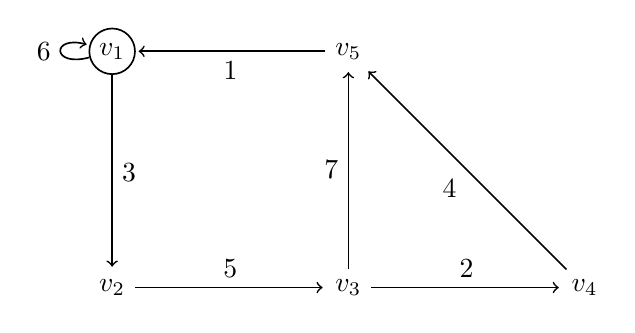
\begin{tikzpicture}[->,shorten >=1pt,auto,node distance=3cm,semithick]

    
      \node[circle, draw, fill=white, inner sep=2pt] (v1) {$v_1$};
      \node (v2) [below of=v1] {$v_2$};
      \node (v3) [right of=v2] {$v_3$};
      \node (v5) [right of=v1] {$v_5$};
      \node (v4) [right of=v5, below of=v5] {$v_4$};
    
      \path (v1) edge node {3} (v2)
            (v2) edge node {5} (v3)
            (v3) edge node {2} (v4)
            (v4) edge node {4} (v5)
            (v5) edge node {1} (v1)
            (v1) edge [loop left] node {6} (v1)
            (v3) edge node {7} (v5);
    \end{tikzpicture}
    \caption{Weighted Directed Graph with 5 Nodes}
\end{figure}

\subsection{Vector spaces}
% Define vector spaces
% Theorems with basis

\subsection{Affine spaces}
% Define affine space
% Define affine combination
% Affine independent vectors yield 

\subsection{Convex Hull}
% Define
% All linear combinations inside Hull are affine combinations

\subsection{Linear Programs}
% Define
% Maybe solving techniques

\subsection{Integer Linear Programs (ILPs)}
% Define
% NP Completeness